% Options for packages loaded elsewhere
\PassOptionsToPackage{unicode}{hyperref}
\PassOptionsToPackage{hyphens}{url}
\documentclass[
]{article}
\usepackage{xcolor}
\usepackage[margin=1in]{geometry}
\usepackage{amsmath,amssymb}
\setcounter{secnumdepth}{-\maxdimen} % remove section numbering
\usepackage{iftex}
\ifPDFTeX
  \usepackage[T1]{fontenc}
  \usepackage[utf8]{inputenc}
  \usepackage{textcomp} % provide euro and other symbols
\else % if luatex or xetex
  \usepackage{unicode-math} % this also loads fontspec
  \defaultfontfeatures{Scale=MatchLowercase}
  \defaultfontfeatures[\rmfamily]{Ligatures=TeX,Scale=1}
\fi
\usepackage{lmodern}
\ifPDFTeX\else
  % xetex/luatex font selection
\fi
% Use upquote if available, for straight quotes in verbatim environments
\IfFileExists{upquote.sty}{\usepackage{upquote}}{}
\IfFileExists{microtype.sty}{% use microtype if available
  \usepackage[]{microtype}
  \UseMicrotypeSet[protrusion]{basicmath} % disable protrusion for tt fonts
}{}
\makeatletter
\@ifundefined{KOMAClassName}{% if non-KOMA class
  \IfFileExists{parskip.sty}{%
    \usepackage{parskip}
  }{% else
    \setlength{\parindent}{0pt}
    \setlength{\parskip}{6pt plus 2pt minus 1pt}}
}{% if KOMA class
  \KOMAoptions{parskip=half}}
\makeatother
\usepackage{color}
\usepackage{fancyvrb}
\newcommand{\VerbBar}{|}
\newcommand{\VERB}{\Verb[commandchars=\\\{\}]}
\DefineVerbatimEnvironment{Highlighting}{Verbatim}{commandchars=\\\{\}}
% Add ',fontsize=\small' for more characters per line
\usepackage{framed}
\definecolor{shadecolor}{RGB}{248,248,248}
\newenvironment{Shaded}{\begin{snugshade}}{\end{snugshade}}
\newcommand{\AlertTok}[1]{\textcolor[rgb]{0.94,0.16,0.16}{#1}}
\newcommand{\AnnotationTok}[1]{\textcolor[rgb]{0.56,0.35,0.01}{\textbf{\textit{#1}}}}
\newcommand{\AttributeTok}[1]{\textcolor[rgb]{0.13,0.29,0.53}{#1}}
\newcommand{\BaseNTok}[1]{\textcolor[rgb]{0.00,0.00,0.81}{#1}}
\newcommand{\BuiltInTok}[1]{#1}
\newcommand{\CharTok}[1]{\textcolor[rgb]{0.31,0.60,0.02}{#1}}
\newcommand{\CommentTok}[1]{\textcolor[rgb]{0.56,0.35,0.01}{\textit{#1}}}
\newcommand{\CommentVarTok}[1]{\textcolor[rgb]{0.56,0.35,0.01}{\textbf{\textit{#1}}}}
\newcommand{\ConstantTok}[1]{\textcolor[rgb]{0.56,0.35,0.01}{#1}}
\newcommand{\ControlFlowTok}[1]{\textcolor[rgb]{0.13,0.29,0.53}{\textbf{#1}}}
\newcommand{\DataTypeTok}[1]{\textcolor[rgb]{0.13,0.29,0.53}{#1}}
\newcommand{\DecValTok}[1]{\textcolor[rgb]{0.00,0.00,0.81}{#1}}
\newcommand{\DocumentationTok}[1]{\textcolor[rgb]{0.56,0.35,0.01}{\textbf{\textit{#1}}}}
\newcommand{\ErrorTok}[1]{\textcolor[rgb]{0.64,0.00,0.00}{\textbf{#1}}}
\newcommand{\ExtensionTok}[1]{#1}
\newcommand{\FloatTok}[1]{\textcolor[rgb]{0.00,0.00,0.81}{#1}}
\newcommand{\FunctionTok}[1]{\textcolor[rgb]{0.13,0.29,0.53}{\textbf{#1}}}
\newcommand{\ImportTok}[1]{#1}
\newcommand{\InformationTok}[1]{\textcolor[rgb]{0.56,0.35,0.01}{\textbf{\textit{#1}}}}
\newcommand{\KeywordTok}[1]{\textcolor[rgb]{0.13,0.29,0.53}{\textbf{#1}}}
\newcommand{\NormalTok}[1]{#1}
\newcommand{\OperatorTok}[1]{\textcolor[rgb]{0.81,0.36,0.00}{\textbf{#1}}}
\newcommand{\OtherTok}[1]{\textcolor[rgb]{0.56,0.35,0.01}{#1}}
\newcommand{\PreprocessorTok}[1]{\textcolor[rgb]{0.56,0.35,0.01}{\textit{#1}}}
\newcommand{\RegionMarkerTok}[1]{#1}
\newcommand{\SpecialCharTok}[1]{\textcolor[rgb]{0.81,0.36,0.00}{\textbf{#1}}}
\newcommand{\SpecialStringTok}[1]{\textcolor[rgb]{0.31,0.60,0.02}{#1}}
\newcommand{\StringTok}[1]{\textcolor[rgb]{0.31,0.60,0.02}{#1}}
\newcommand{\VariableTok}[1]{\textcolor[rgb]{0.00,0.00,0.00}{#1}}
\newcommand{\VerbatimStringTok}[1]{\textcolor[rgb]{0.31,0.60,0.02}{#1}}
\newcommand{\WarningTok}[1]{\textcolor[rgb]{0.56,0.35,0.01}{\textbf{\textit{#1}}}}
\usepackage{longtable,booktabs,array}
\usepackage{calc} % for calculating minipage widths
% Correct order of tables after \paragraph or \subparagraph
\usepackage{etoolbox}
\makeatletter
\patchcmd\longtable{\par}{\if@noskipsec\mbox{}\fi\par}{}{}
\makeatother
% Allow footnotes in longtable head/foot
\IfFileExists{footnotehyper.sty}{\usepackage{footnotehyper}}{\usepackage{footnote}}
\makesavenoteenv{longtable}
\usepackage{graphicx}
\makeatletter
\newsavebox\pandoc@box
\newcommand*\pandocbounded[1]{% scales image to fit in text height/width
  \sbox\pandoc@box{#1}%
  \Gscale@div\@tempa{\textheight}{\dimexpr\ht\pandoc@box+\dp\pandoc@box\relax}%
  \Gscale@div\@tempb{\linewidth}{\wd\pandoc@box}%
  \ifdim\@tempb\p@<\@tempa\p@\let\@tempa\@tempb\fi% select the smaller of both
  \ifdim\@tempa\p@<\p@\scalebox{\@tempa}{\usebox\pandoc@box}%
  \else\usebox{\pandoc@box}%
  \fi%
}
% Set default figure placement to htbp
\def\fps@figure{htbp}
\makeatother
\setlength{\emergencystretch}{3em} % prevent overfull lines
\providecommand{\tightlist}{%
  \setlength{\itemsep}{0pt}\setlength{\parskip}{0pt}}
\usepackage{bookmark}
\IfFileExists{xurl.sty}{\usepackage{xurl}}{} % add URL line breaks if available
\urlstyle{same}
\hypersetup{
  pdftitle={Monte Carlo Estimation of π on HTCondor},
  pdfauthor={Snikitha Siddavatam},
  hidelinks,
  pdfcreator={LaTeX via pandoc}}

\title{Monte Carlo Estimation of π on HTCondor}
\usepackage{etoolbox}
\makeatletter
\providecommand{\subtitle}[1]{% add subtitle to \maketitle
  \apptocmd{\@title}{\par {\large #1 \par}}{}{}
}
\makeatother
\subtitle{Understanding Throughput Using a Standardized Workflow}
\author{Snikitha Siddavatam}
\date{July 10, 2026}

\begin{document}
\maketitle

{
\setcounter{tocdepth}{3}
\tableofcontents
}
\section{Objective}\label{objective}

Profile the error of Monte Carlo numerical integration as an estimator
of π as a function of the total number of samples \emph{N}. By
submitting \emph{J} independent HTCondor jobs, each producing a fixed
number of samples \emph{S}, and accumulating results in chronological
order of job completion, we observe how the absolute estimation error
decreases as \emph{N} grows --- and how job throughput and turnaround
behave as \emph{J} scales from 10 to 100,000.

\section{Background}\label{background}

The Monte Carlo method estimates π by exploiting the ratio of the area
of a unit circle to its enclosing unit square. For a point \((x, y)\)
drawn uniformly from \([0,1) \times [0,1)\), the point falls inside the
quarter-circle if:

\[x^2 + y^2 < 1\]

The fraction of points satisfying this condition converges to \(\pi/4\)
as the number of samples grows. Multiplying by 4 gives the estimate of
π. The expected error decreases proportionally to \(1/\sqrt{N}\) (the
standard Monte Carlo convergence rate).

\section{Experiment Parameters}\label{experiment-parameters}

\begin{longtable}[]{@{}
  >{\raggedright\arraybackslash}p{(\linewidth - 4\tabcolsep) * \real{0.3438}}
  >{\raggedright\arraybackslash}p{(\linewidth - 4\tabcolsep) * \real{0.2500}}
  >{\raggedright\arraybackslash}p{(\linewidth - 4\tabcolsep) * \real{0.4062}}@{}}
\toprule\noalign{}
\begin{minipage}[b]{\linewidth}\raggedright
Parameter
\end{minipage} & \begin{minipage}[b]{\linewidth}\raggedright
Symbol
\end{minipage} & \begin{minipage}[b]{\linewidth}\raggedright
Description
\end{minipage} \\
\midrule\noalign{}
\endhead
\bottomrule\noalign{}
\endlastfoot
Samples per job & S & Fixed number of random points generated by a
single job \\
Number of jobs & J & Total jobs submitted; controls total samples N = S
× J \\
Total samples & N & Cumulative sample count after j jobs: N = S × j \\
Reference value of π & π\_ref & High-precision reference,
3.14159265358979323846\ldots{} \\
Absolute error & ε & \textbar π\_estimated − π\_ref\textbar{} \\
\end{longtable}

\section{Job Design}\label{job-design}

Each HTCondor job is a self-contained execution unit that:

\begin{itemize}
\tightlist
\item
  Sets the random seed based on the job number (ProcID) and cluster
  number (ClusterID)
\item
  Generates exactly S random \((x, y)\) pairs uniformly distributed in
  \([0,1) \times [0,1)\)
\item
  Counts the number of points M satisfying \(x^2 + y^2 < 1\)
\item
  Computes a local estimate: \(\pi_{local} = 4M/S\)
\item
  Writes a single output file to the Access Point upon completion (the
  script writes no output if it errors)
\item
  Sleeps for a duration (1--60s) \textbf{assigned at submit time} before
  exiting, to stagger completion times (see \emph{Sleep-time assignment}
  under \emph{Next Steps})
\end{itemize}

A job is considered \textbf{done} if and only if its output file exists
at the Access Point \emph{and} there is a corresponding
\texttt{JOB\_TERMINATED} entry for that Job ID in the HTCondor log. All
jobs within an experiment request identical CPU, memory, disk,
clock-time limit, and execution environment, so differences in
completion time reflect scheduling and pool variation rather than
resource differences.

\subsection{\texorpdfstring{Worker script:
\texttt{mc\_pi.py}}{Worker script: mc\_pi.py}}\label{worker-script-mc_pi.py}

\begin{Shaded}
\begin{Highlighting}[]
\NormalTok{python mc\_pi.py }\OperatorTok{\textless{}}\NormalTok{S}\OperatorTok{\textgreater{}} \OperatorTok{\textless{}}\NormalTok{ProcID}\OperatorTok{\textgreater{}} \OperatorTok{\textless{}}\NormalTok{ClusterID}\OperatorTok{\textgreater{}}
\end{Highlighting}
\end{Shaded}

\textbf{How seeding works:} the seed is derived from
\texttt{MD5(ClusterID\_ProcID)} mapped to a 32-bit integer, guaranteeing
that no two \texttt{(ClusterID,\ ProcID)} pairs share a seed --- every
job produces statistically independent samples, even across multiple
submission clusters.

\textbf{Output} (\texttt{output\_\textless{}ProcID\textgreater{}.txt}):

\begin{verbatim}
job_id=<ProcID>
cluster_id=<ClusterID>
seed=<seed>
samples=<S>
hits=<M>
pi_estimate=<4*M/S>
\end{verbatim}

\subsection{\texorpdfstring{Submit file:
\texttt{mc\_pi.sub}}{Submit file: mc\_pi.sub}}\label{submit-file-mc_pi.sub}

Submits \emph{J} independent jobs to HTCondor, each running
\texttt{mc\_pi.py\ \textless{}S\textgreater{}\ \$(Process)\ \$(Cluster)}.
With submit-side sleep assignment, the submit file queues from the
pregenerated job-parameter table
(\texttt{queue\ sleep\_time\ from\ \textless{}table\textgreater{}}) so
each job's sleep duration arrives as an argument. Output, error, and log
files are organized per-cluster under \texttt{run\_\$(Cluster)/logs/},
and result files are transferred back and remapped into the same folder.

\section{Pipeline}\label{pipeline}

\begin{verbatim}
1. condor_submit mc_pi.sub                → run_<ClusterID>/ created
2. condor_wait .../mc_pi.log               → wait for all jobs to terminate
3. mv run_<ClusterID> mc_runs_<J>/         → file under the right job-count bucket
4. python make_graphs.py <J>               → aggregate + plot in one step
5. python milestone_times.py               → percentile completion times, all job counts
6. python milestone_scatter.py             → milestone comparison plots
\end{verbatim}

\texttt{make\_graphs.py} (parameterized by job count \texttt{J}):

\begin{enumerate}
\def\labelenumi{\arabic{enumi}.}
\tightlist
\item
  Aggregates any \texttt{run\_*} folders in
  \texttt{mc\_runs\_\textless{}J\textgreater{}/} lacking a
  \texttt{results.csv}: parses each
  \texttt{output\_\textless{}job\_id\textgreater{}.txt},
  cross-references the HTCondor log for termination timestamps, keeps
  only jobs with both a valid output file and a \texttt{JOB\_TERMINATED}
  entry, sorts by completion time, and computes running cumulative π
  estimate and absolute error.
\item
  Produces four plots per run under
  \texttt{graphs/\textless{}J\textgreater{}\_jobs/}:

  \begin{itemize}
  \tightlist
  \item
    \texttt{mc\_runs\_\textless{}J\textgreater{}\_scatter.png} --- π
    estimate vs.~cumulative jobs, and log-log error vs.~N
  \item
    \texttt{mc\_runs\_\textless{}J\textgreater{}\_runtime.png} ---
    cumulative samples vs.~wall-clock time
  \item
    \texttt{mc\_runs\_\textless{}J\textgreater{}\_runtime\_jobs.png} ---
    cumulative jobs completed vs.~wall-clock time
  \item
    \texttt{mc\_runs\_\textless{}J\textgreater{}\_turnaround.png} ---
    per-job turnaround time vs.~Job ID
  \end{itemize}
\end{enumerate}

\texttt{results.csv} columns: \texttt{j}, \texttt{job\_id},
\texttt{submit\_time}, \texttt{timestamp}, \texttt{turnaround\_s},
\texttt{N}, \texttt{pi\_est}, \texttt{error}.

\section{Results}\label{results}

Experiments were run at five scales: \textbf{10, 100, 1,000, 10,000, and
100,000} jobs, each with S = 10,000 samples per job.

\subsection{Cross-scale comparison}\label{cross-scale-comparison}

To compare throughput across job counts on a common footing,
\texttt{milestone\_times.py} records the wall-clock time (from first job
completion) at which each 10\% completion milestone was reached, for
every run at every job count, and \texttt{milestone\_scatter.py} plots
the pooled results.

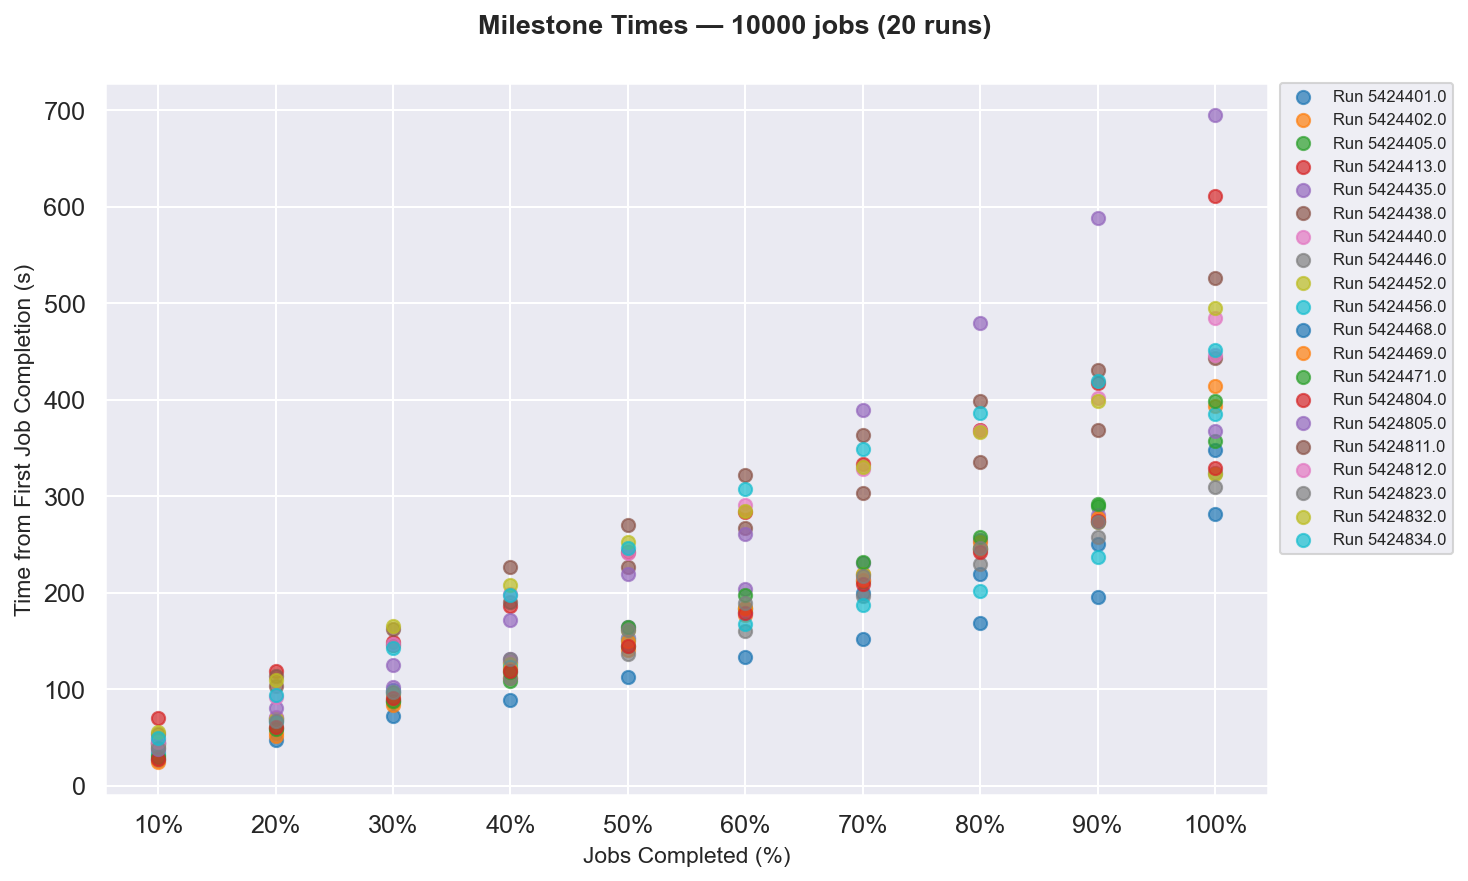
\includegraphics[width=1\linewidth]{graphs/milestones/milestones_10000_jobs}

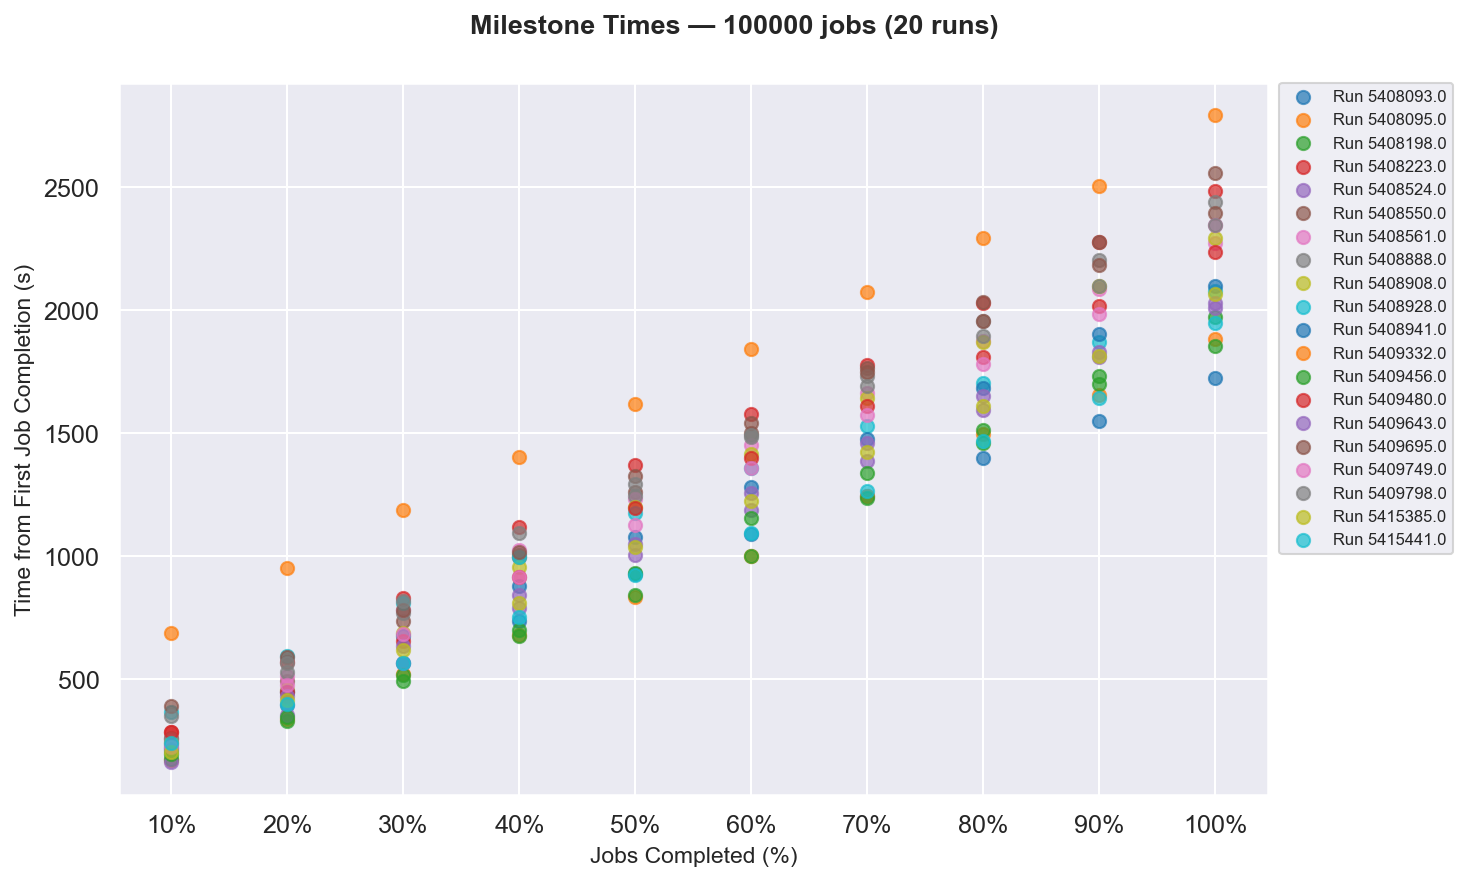
\includegraphics[width=1\linewidth]{graphs/milestones/milestones_100000_jobs}

\section{\texorpdfstring{Files in
\texttt{monte\_carlo\_pi/}}{Files in monte\_carlo\_pi/}}\label{files-in-monte_carlo_pi}

\begin{longtable}[]{@{}
  >{\raggedright\arraybackslash}p{(\linewidth - 2\tabcolsep) * \real{0.5000}}
  >{\raggedright\arraybackslash}p{(\linewidth - 2\tabcolsep) * \real{0.5000}}@{}}
\toprule\noalign{}
\begin{minipage}[b]{\linewidth}\raggedright
File
\end{minipage} & \begin{minipage}[b]{\linewidth}\raggedright
Role
\end{minipage} \\
\midrule\noalign{}
\endhead
\bottomrule\noalign{}
\endlastfoot
\texttt{mc\_pi.py} & Worker script: generates S samples, writes
\texttt{output\_\textless{}ProcID\textgreater{}.txt} \\
\texttt{mc\_pi.sub} & HTCondor submit file (\texttt{queue\ J}) \\
\texttt{aggregate.py} & Original aggregation script (reads
\texttt{mc\_runs/}) \\
\texttt{graph.py} & Original convergence plot script (reads
\texttt{mc\_runs/}) \\
\texttt{runtime\_graph.py} & Runtime + turnaround plots (reads
\texttt{mc\_runs/}, the original 100-job experiment) \\
\texttt{make\_graphs.py} & All-in-one aggregate + plot, parameterized by
job count \\
\texttt{milestone\_times.py} & Extracts percentile completion times
across all job counts → \texttt{milestone\_times.csv} \\
\texttt{milestone\_scatter.py} & Plots \texttt{milestone\_times.csv} \\
\texttt{utils.py} & Shared helper: \texttt{get\_run\_folders()} \\
\texttt{examples/} & Sample output files + parse test, for testing
without HTCondor \\
\end{longtable}

\section{Caveats}\label{caveats}

\begin{quote}
Running a large number of jobs can impact user priority relative to
other users on the pool, reducing throughput via fair-share balancing.
For reproducible comparisons across scales, user priority should be
reset between runs.
\end{quote}

\section{Next Steps}\label{next-steps}

\subsection{Sleep-time assignment: submit-side seed
chain}\label{sleep-time-assignment-submit-side-seed-chain}

Rather than letting each job pick its own seed for the sleep duration,
the sleep times are generated \textbf{once, on the submit side}, and
passed to each job as an explicit parameter. This keeps the full
experiment under our control and makes every run exactly reproducible
from a single starting seed.

The seeds form a deterministic chain via a recurrence:

\[R_i = f(R_{i-1})\]

Starting from a single initial seed \(R_0\), the recurrence is applied
repeatedly to produce one value per job - e.g.~100,000 values for a
100,000-job run. Each \(R_i\) is then mapped to a sleep duration in the
1--60 s range and written into a job-parameter table. The submit file
iterates over this table
(\texttt{queue\ sleep\_time\ from\ \textless{}table\textgreater{}}), so
each job receives its sleep duration as an argument instead of computing
it internally.

Why this matters:

\begin{itemize}
\tightlist
\item
  \textbf{Control:} the submitter, not the job, decides every sleep
  time; the experiment's completion-time staggering is fully specified
  before any job runs.
\item
  \textbf{Reproducibility:} one starting seed \(R_0\) regenerates the
  entire sequence of sleep times, for any number of jobs.
\item
  \textbf{Independence from the sampling seed:} the Monte Carlo sampling
  seed (derived from \texttt{ClusterID}/\texttt{ProcID}) and the sleep
  duration are decoupled, so changing the staggering scheme never
  perturbs the π estimates.
\end{itemize}

\subsection{Memory Profiling}\label{memory-profiling}

We observed that users are requesting a lot of memory while running jobs
and it takes longer for jobs to move through the system.
\textbf{Understanding how throughput changes with memory requests.}

Why do we care about memory?

\begin{itemize}
\tightlist
\item
  Ask for too much → fewer machines can fit your job → longer waits
\item
  Ask for too little → job can get kicked off or put on hold
\item
  So memory requests directly change how many jobs finish per hour
\end{itemize}

What we'll do:

\begin{itemize}
\tightlist
\item
  Run the same workload with different memory requests, varying
  \texttt{request\_memory} for each run from \textbf{500 MB to 64 GB}
\item
  Measure how throughput changes
\end{itemize}

\end{document}
